\chapter{Methodology}

The first part of this chapter describes the data sources: datasets based on administrations of Ordered-Multiple Choice (OMC) items written to assess student understanding relative to the (1) Earth and Solar System and (2) Force and Motion learning progressions. The second part will detail how I will address the two research questions by using three models presented in the previous chapter; a) the Partial Credit Model \cite{Masters1982,EmbretsonReise2000}, b) the Attribute Hierarchy Method (as modified by \citeNP{BriggsAlonzo2012} ) for use with OMC items, and c) the General Diagnostic Model \cite{vonDavier2008}. It will likewise present the challenges that the use of OMC items can create for the diagnostic modeling.

\section{\em The ESS and FM Learning Progressions}
This study uses empirical data from two learning progressions. The first is a LP for "Earth and Solar System" (ESS), previously presented in the introduction chapter. A total of 12 items were developed to assess students' understanding of three different phenomena within the ESS domain; (a) the day/night cycle, (b) the phases of the Moon, and (c) the seasons-in terms of the motion of objects in the Solar System \cite{Briggs2006}. The second LP focuses on the concept of Forces and Motion (FM).  A total of 16 items were developed \cite{AlonzoSteedle2009} to assess students' understanding of one-dimensional forces (e.g., downward gravitational force represented on - y axis in Cartesian coordinate system) and resulting motion. This LP describes the growth of students' understanding across five levels from no evidence on student understanding of concepts, to an "expert" level of understanding the relationship between force and acceleration (i.e. change in speed or direction). Each LP level includes the descriptions of student thinking on the objects' behaviors in the cases of force/no force and motion/no motion \cite[p.~403-404]{AlonzoSteedle2009}. In a similar way to the ESS LP, this learning progression is developed using the science standards defined for understanding of force and motion expected of eighth-grade students and related researched on student conceptions/misconceptions \cite{AlonzoSteedle2009}. 
Both LP assessments were administered to a sample of 1008 high school students at six schools in rural and suburban Iowa during the 2008-09 school year within one test including 28 items. The schools and teachers that agreed to administer the assessment were a convenience sample. As noted by \citeA{BriggsAlonzo2012}, the reason for choosing high school students for the study was to minimize guessing based on the claim that most high school students should have been exposed to the ideas in the two learning progressions and therefore would not need to guess at answers. As a consequence, such students are less likely to consistently choose responses consistent with lower levels of functioning on the LP.  
According to \citeA[p.~4-5]{BriggsAlonzo2012} , the average participation rate across all classes was fairly high at 83\%. Almost half of the sample (48\%) was female students. Students were also asked whether content of assessment questions covered in any science class they have taken. 46\% of students responded "yes," another 25\% answered "no", 28\% answered "I am not sure" and 2\% did not respond at all.

\section{\em Ordered Multiple-Choice Items}

Both LP assessments consisted of Ordered-Multiple Choice (OMC) items. OMC items look like traditional multiple choice items; however, they contain item options which reflect the different learning progression levels. That means that although one of the options is the most correct response, based on the fact that it is linked to the highest level of the progression, other options connected to lower levels of progression are not entirely incorrect and they are designed to provide information about the ways that students might be thinking about the relationships between the relevant concepts. Because OMC items build on the cognitive differences specified in learning progression levels into the item options, they tend to offer more valid and reliable results \cite<e.g.,>{AlonzoSteedle2009,Briggs2006}. One OMC item example from each LP is presented in the following figure.

\begin{figure}[htbp]
  \centering
  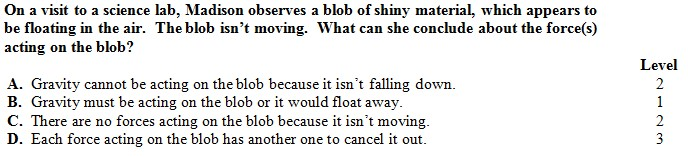
\includegraphics[width=\textwidth]{figs/OMC1.jpg}
  \caption{Example Ordered Multiple Choice Item:Motion}
  \label{fig:OMC1}
\end{figure}

The item presented in Figure  ~\ref{fig:OMC1} on page ~\pageref{fig:OMC1} asks about the foces acting on a blob and it has 3 LP levels associated with 4 options. 


\begin{figure}[htbp]
  \centering
  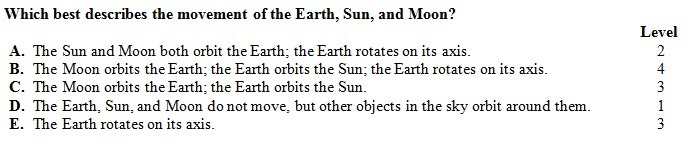
\includegraphics[width=\textwidth]{figs/OMC2.jpg}
  \caption{Example Ordered Multiple Choice Item:Force\label{fig:OMC2}}
 \end{figure}

The item in the Figure ~\ref{fig:OMC2} asks about the movement of Sun, Earth and Moon. It has 5 options associated with 4 LP levels. 


All item options in Figure %\ref{OMC1} and %\ref{OMC2}%
 are linked to the learning progression levels. That is, the polytomous scoring of items are intended to capture the LP levels. Note however, the complication that there can be a many to one link between a response options and an LP level. 


\subsection{Item Response Theory Model}

My strategy to use the IRT modeling is similar to the ones used in the literature with Partial Credit Model (PCM). Next, I will present the PCM \cite{Masters1982,EmbretsonReise2000} which is an extension of the Rasch model.

Consider a response from individual $j$ to item $i$ that has been coded as polytomously,representing the multiple response categories. 

This model is a divide-by-sum model where the probability of a response in each category is defined as an exponential divided by sum of exponentials. For a polytomous item with $K_{i} = 1+m_{i}$ categories which are scored $x= 0,\dots,m_{i}$, the probability of selecting response level $j$ for an ability level of theta is done.

If an entire set of items depends upon only a single latent trait, then the probability of a correct response can be parametrized as:



\begin{equation}
P_{i}(x=j|theta)=\frac{\text{exp}\big[\sum_{j=0}^x(\theta_j-\delta_{ij})]}{\sum_{r=0}^{m_i} \big[\text{exp}\sum_{j=0}^r(\theta_j-\delta_{ij})]} \label{PCM}.
\end{equation}

